%%%%%%%%%%%%%%%%%Epic 7, 8, 9, 10%%%%%%%%%%%%%%%%%%%%%%%%%%%%%%%%%%%%%%%%%%%%%%%%%%%%%%%

\subsection{Objekte erkennen}

Dieses Kapitel behandelt die Methoden zur Objekterkennung. Zur Identifikation von Objekten auf dem Graphen, wurde ein YOLOv11-Modell eingesetzt, das speziell für diese Aufgabe trainiert wurde. Die erzielten Modellresultate werden vom Raspberry Pi ausgewertet, damit der Roboter die optimale Route wählen kann. Ergänzend dazu dient ein Ultraschallsensor als Backup-System zur Erkennung von Hindernissen, um die Sicherheit des Roboters zu erhöhen. 


\subsubsection{Ultraschall}
\label{ultraschall}

Es gibt eine Backup-Hinderniserkennung mittels Ultraschallsensor, um Risiko 12 (Objekte werden nicht erkannt) zu Minimieren.

Zur Erhöhung der Betriebssicherheit ist das Fahrzeug mit einer redundanten Hinderniserkennung ausgestattet. Diese erfolgt über einen Ultraschallsensor, der kontinuierlich die Entfernung zu Objekten im unmittelbaren Umfeld misst. Der Sensor ist direkt mit dem Mikrocontroller \gls{tinyk22} verbunden.

Die Messwerte werden in Echtzeit ausgewertet. Sobald ein Objekt in einer Distanz von weniger als 10 cm erkannt wird, wird automatisch ein Not-Stopp ausgelöst, um Kollisionen zu vermeiden. Gleichzeitig wird ein definierter Fehlercode generiert und über eine serielle Schnittstelle an den Raspberry Pi übertragen, um den Fehlerstatus zu protokollieren und entsprechende Massnahmen einleiten zu können. Dies ist beschrieben in Tabelle \ref{table:statuscodes}.


QUESTION: TODO IVAN MORE INFO ABOUT HOW TO READ 

TODO ELIAS MORE INFO ABOUT WHERE/HOW ADDED 




\subsubsection{YOLOv11-Model trainieren}

Damit der Roboter Pylonen, Knoten und Hindernissen erkennen kann, wurde ein \gls{yolo} Model trainiert.
Es wurden mehrere Models trainiert, die laufend miteinander verglichen wurden. Der Prozess wie das finale Model gewählt wurde, ist im Anhang in Kapitel \nameref{model-evaluation} zu finden.

Das Model, das verwendet werden wird, deutet die Bilder in ihrer Originalgrsse und hat über alle Klassen (Pylonen, Knoten, Hindernisse) gute Ergebnisse.

Die folgenden Bilder zeigen einige Bilder, die das Model annotiert hat. Darauf ist zu sehen, wie genau es die einzelnen Objekte erkennen kann.

\begin{figure}[H]
  \centering
    \begin{minipage}[b]{0.28\textwidth}
    \centering
    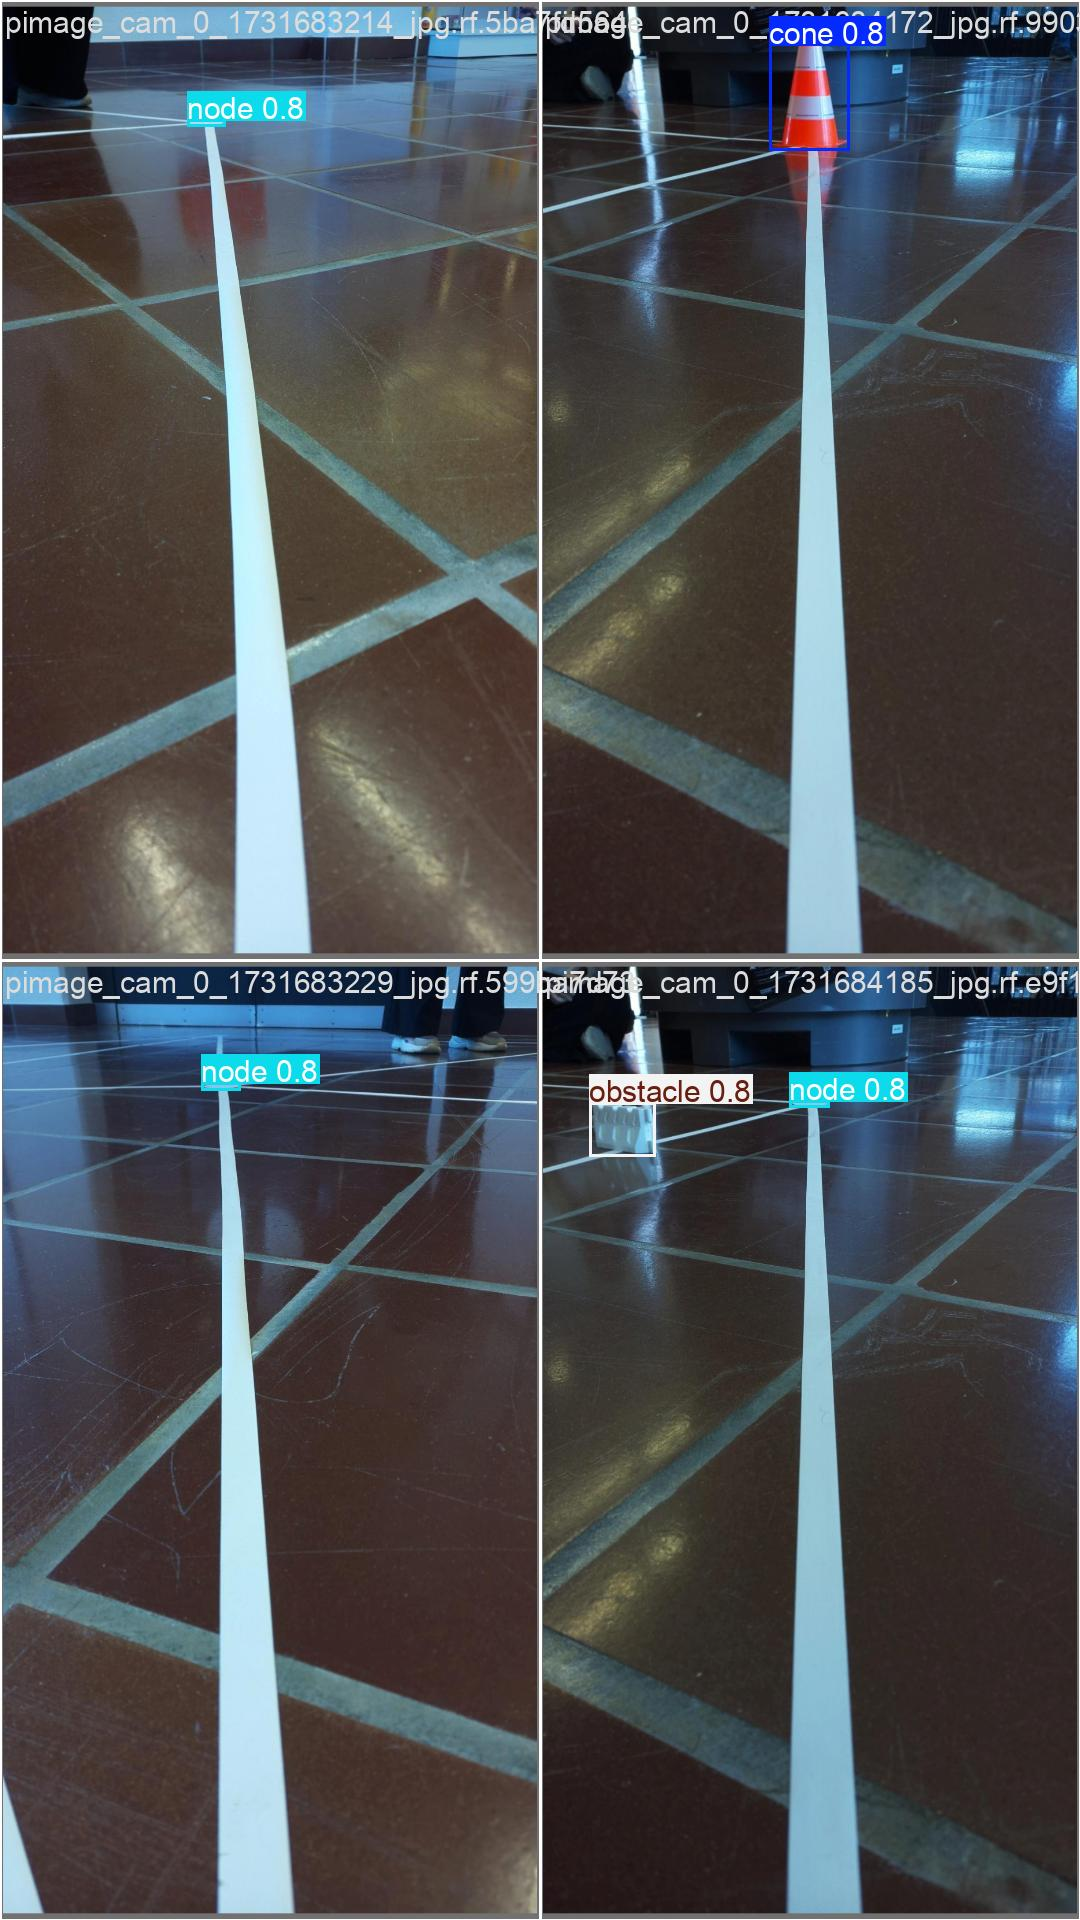
\includegraphics[width=\textwidth]{assets/IT/yolo/val_batch0_pred.jpg}
    \caption{Bilderkennung I}
    \label{fig:yolo-i}
  \end{minipage}
  \hfill
  \begin{minipage}[b]{0.28\textwidth}
    \centering
    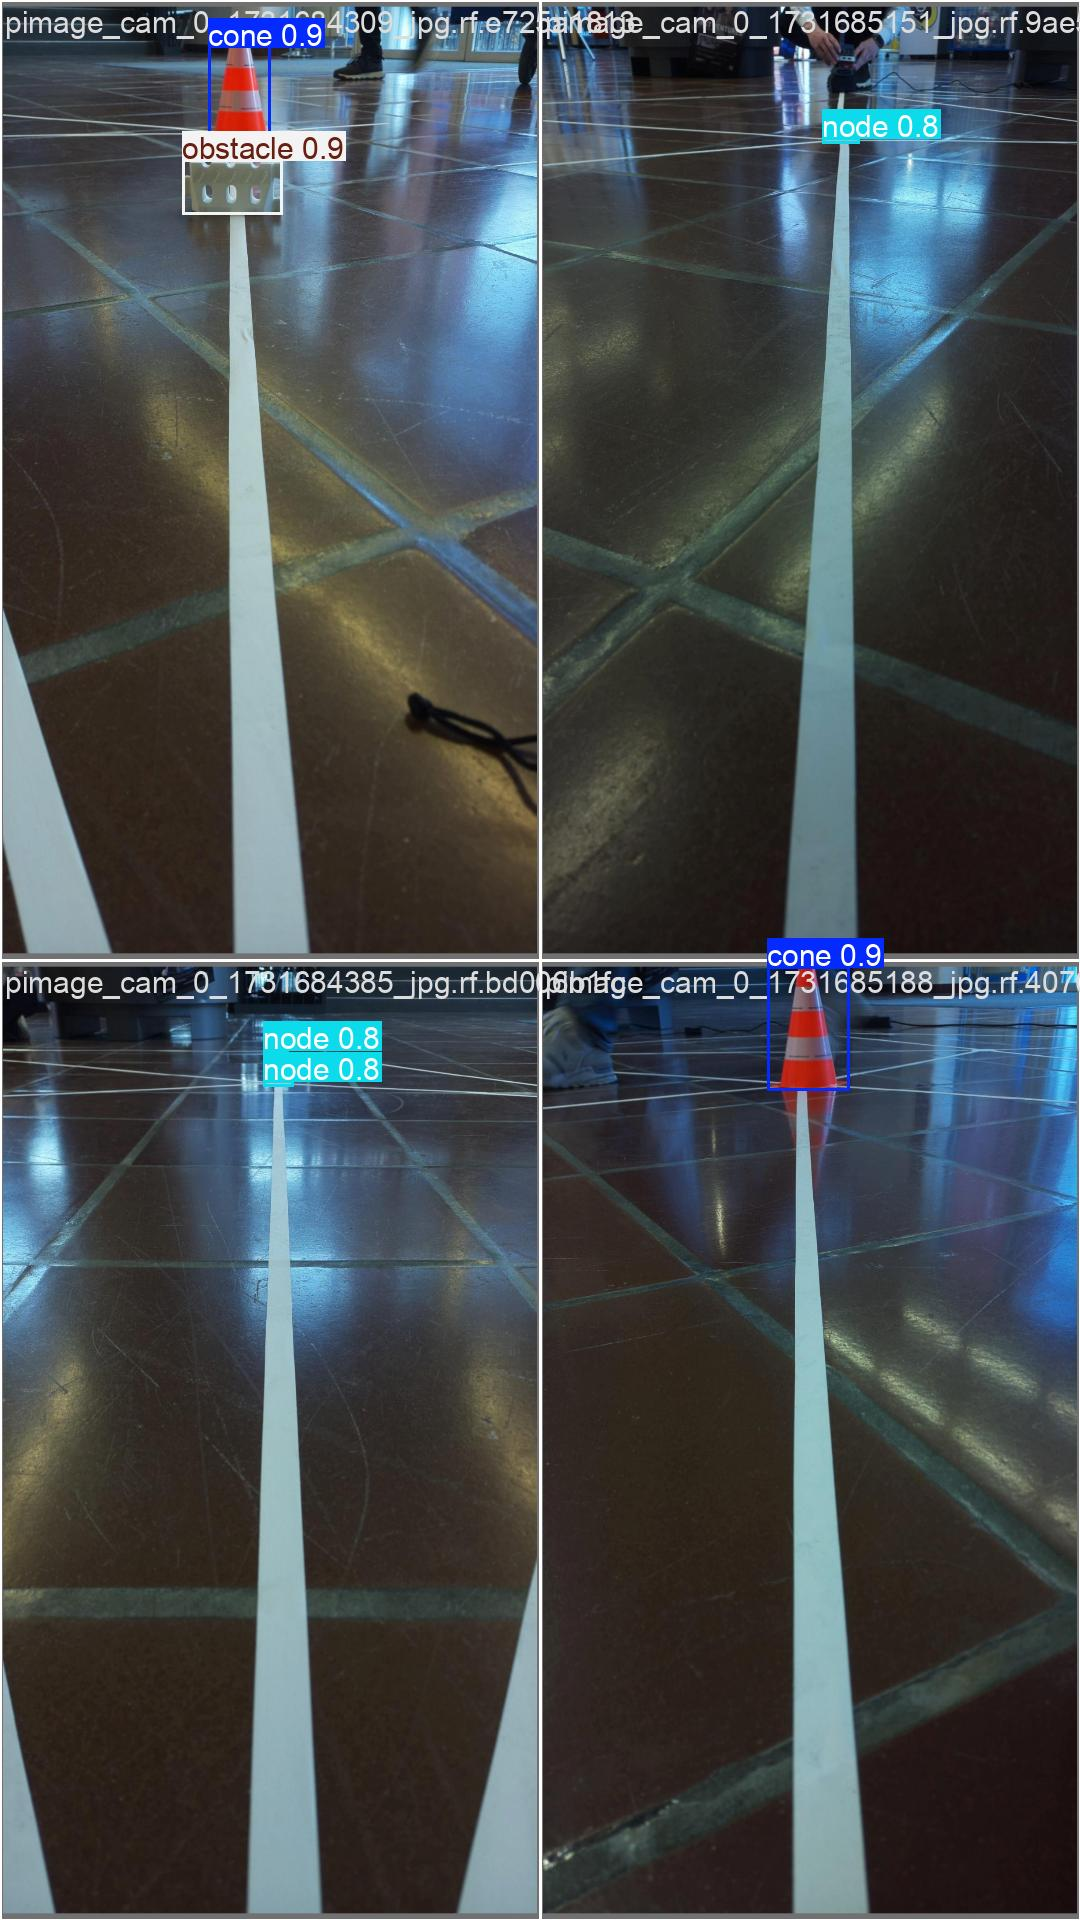
\includegraphics[width=\textwidth]{assets/IT/yolo/val_batch1_pred.jpg}
    \caption{Bilderkennung II}
    \label{fig:yolo-ii}
  \end{minipage}
    \hfill
  \begin{minipage}[b]{0.28\textwidth}
    \centering
    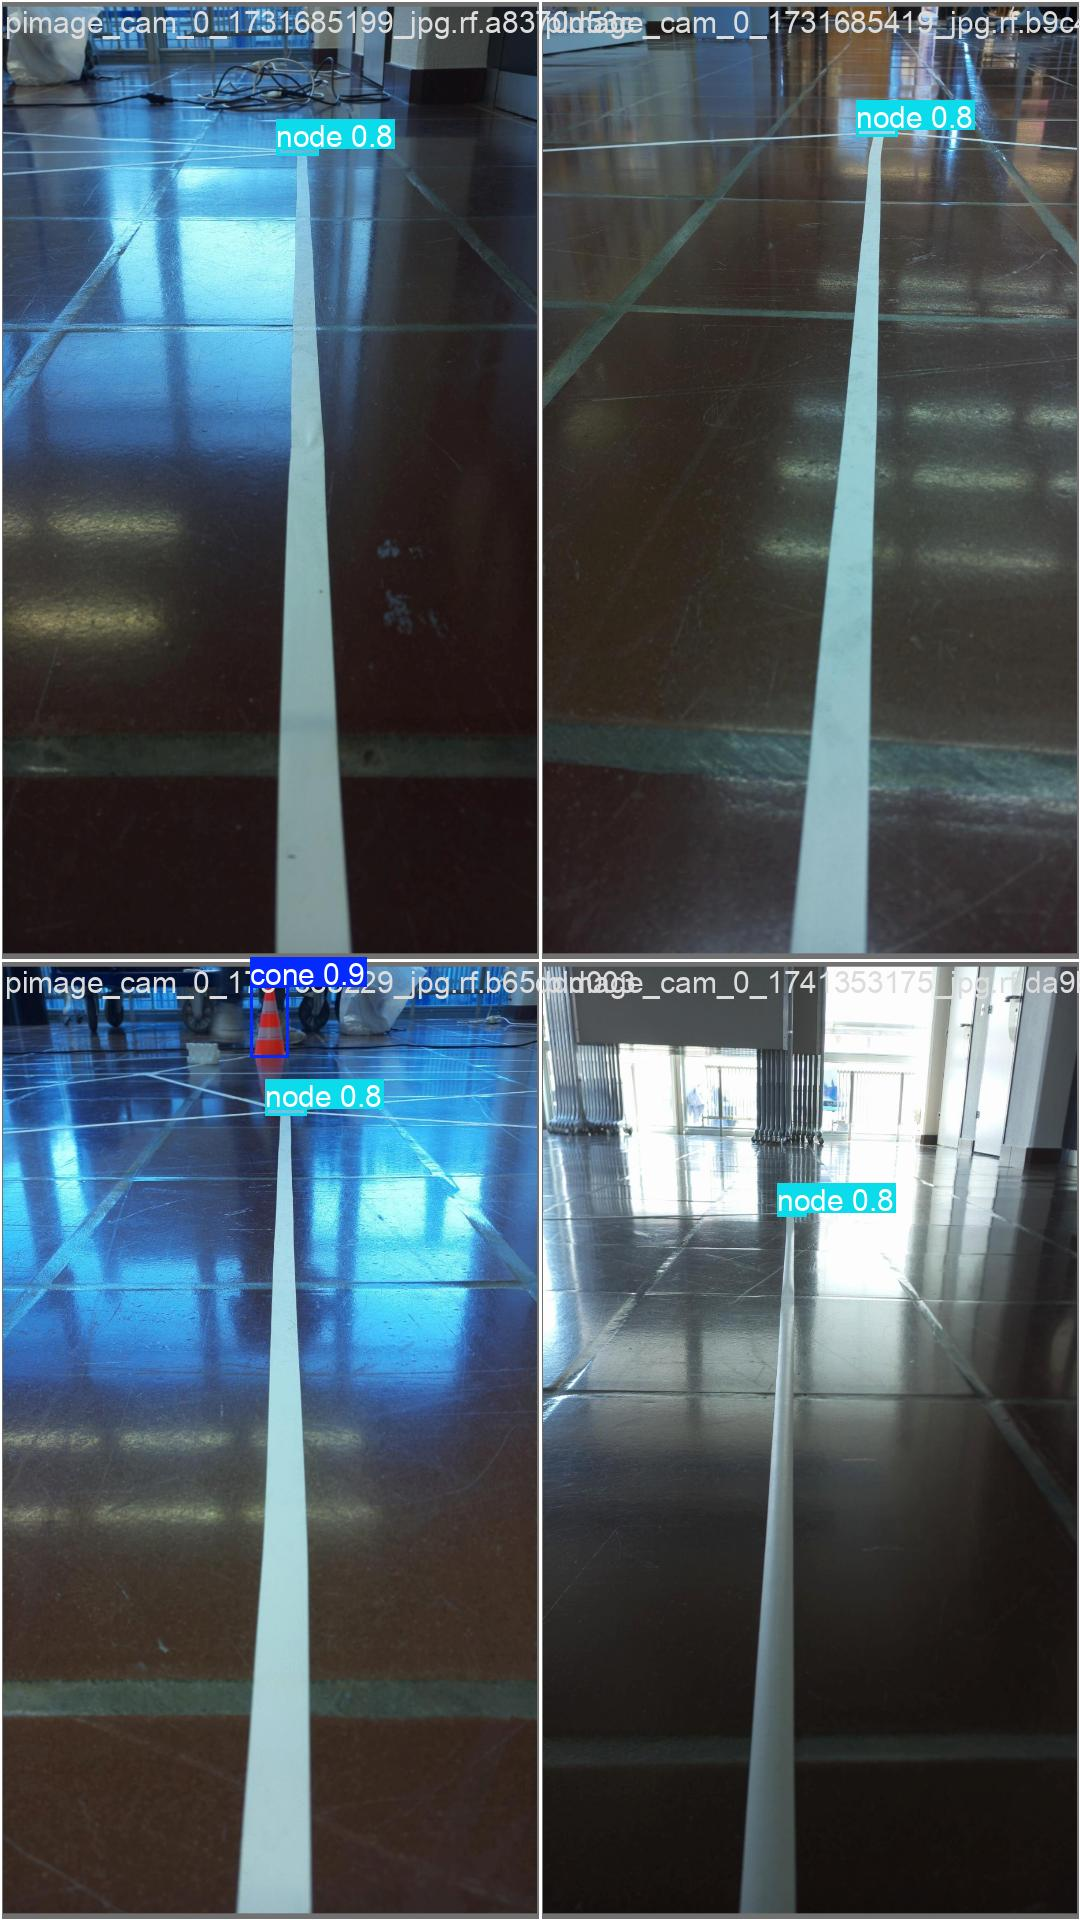
\includegraphics[width=\textwidth]{assets/IT/yolo/val_batch2_pred.jpg}
    \caption{Bilderkennung III}
    \label{fig:yolo-iii}
  \end{minipage}
\end{figure}

Auf den folgenden Bildern sind die Metriken aufgezeigt. Diese sind ebenfalls im Anhang im Kapitel \nameref{model-evaluation} genauer erklaert. Was hier sichtbar ist, ist zum einen der F1 Wert. Dieser ist besser, je höher er ist. Er ist hier fuer alle Klassen sehr hoch, was auf eine hohe Genauigkeit in den Detekierungen deutet. Ebenfalls ist die Consuion Matrix erkenntlich, diese zeigt welche Objekte das Model wie oft falsch oder richtig gedeutet hat. Das Model hat jede Pylone erkannt, hat sich zwei Knoten eingebildet und zwei Knoten verpasst. Mit den Algorithmen, die in dem nachfolgenden Kapitel \ref{model-results} beschrieben sind, die die Modelperformance stuetzen, sind diese Resultate ausgezeichnet. Ebenfalls ist der Lernverlauf des Models ersichtlich. Alle Graphen zeigen das gewünschte Muster. Die 6 Graphen links, die den Verlust in der Leistung (falsche Deutungen) darstellen, sind exponentiell fallend. Das heisst, dass das Modell mit jeder Iteration mehr gelernt hat und nicht irgendwann gestoppt hat oder schlechter wurde. Die 4 Graphen auf der rechten Seite zeigen, wie viel das Model gelernt, diese steigen und flachen dann ab. Dies ist ebenfalls das Muster, das bei einem guten Model erwartet wird.\cite{model-performance}

\begin{figure}[H]
  \centering
    \begin{minipage}[b]{0.3\textwidth}
    \centering
    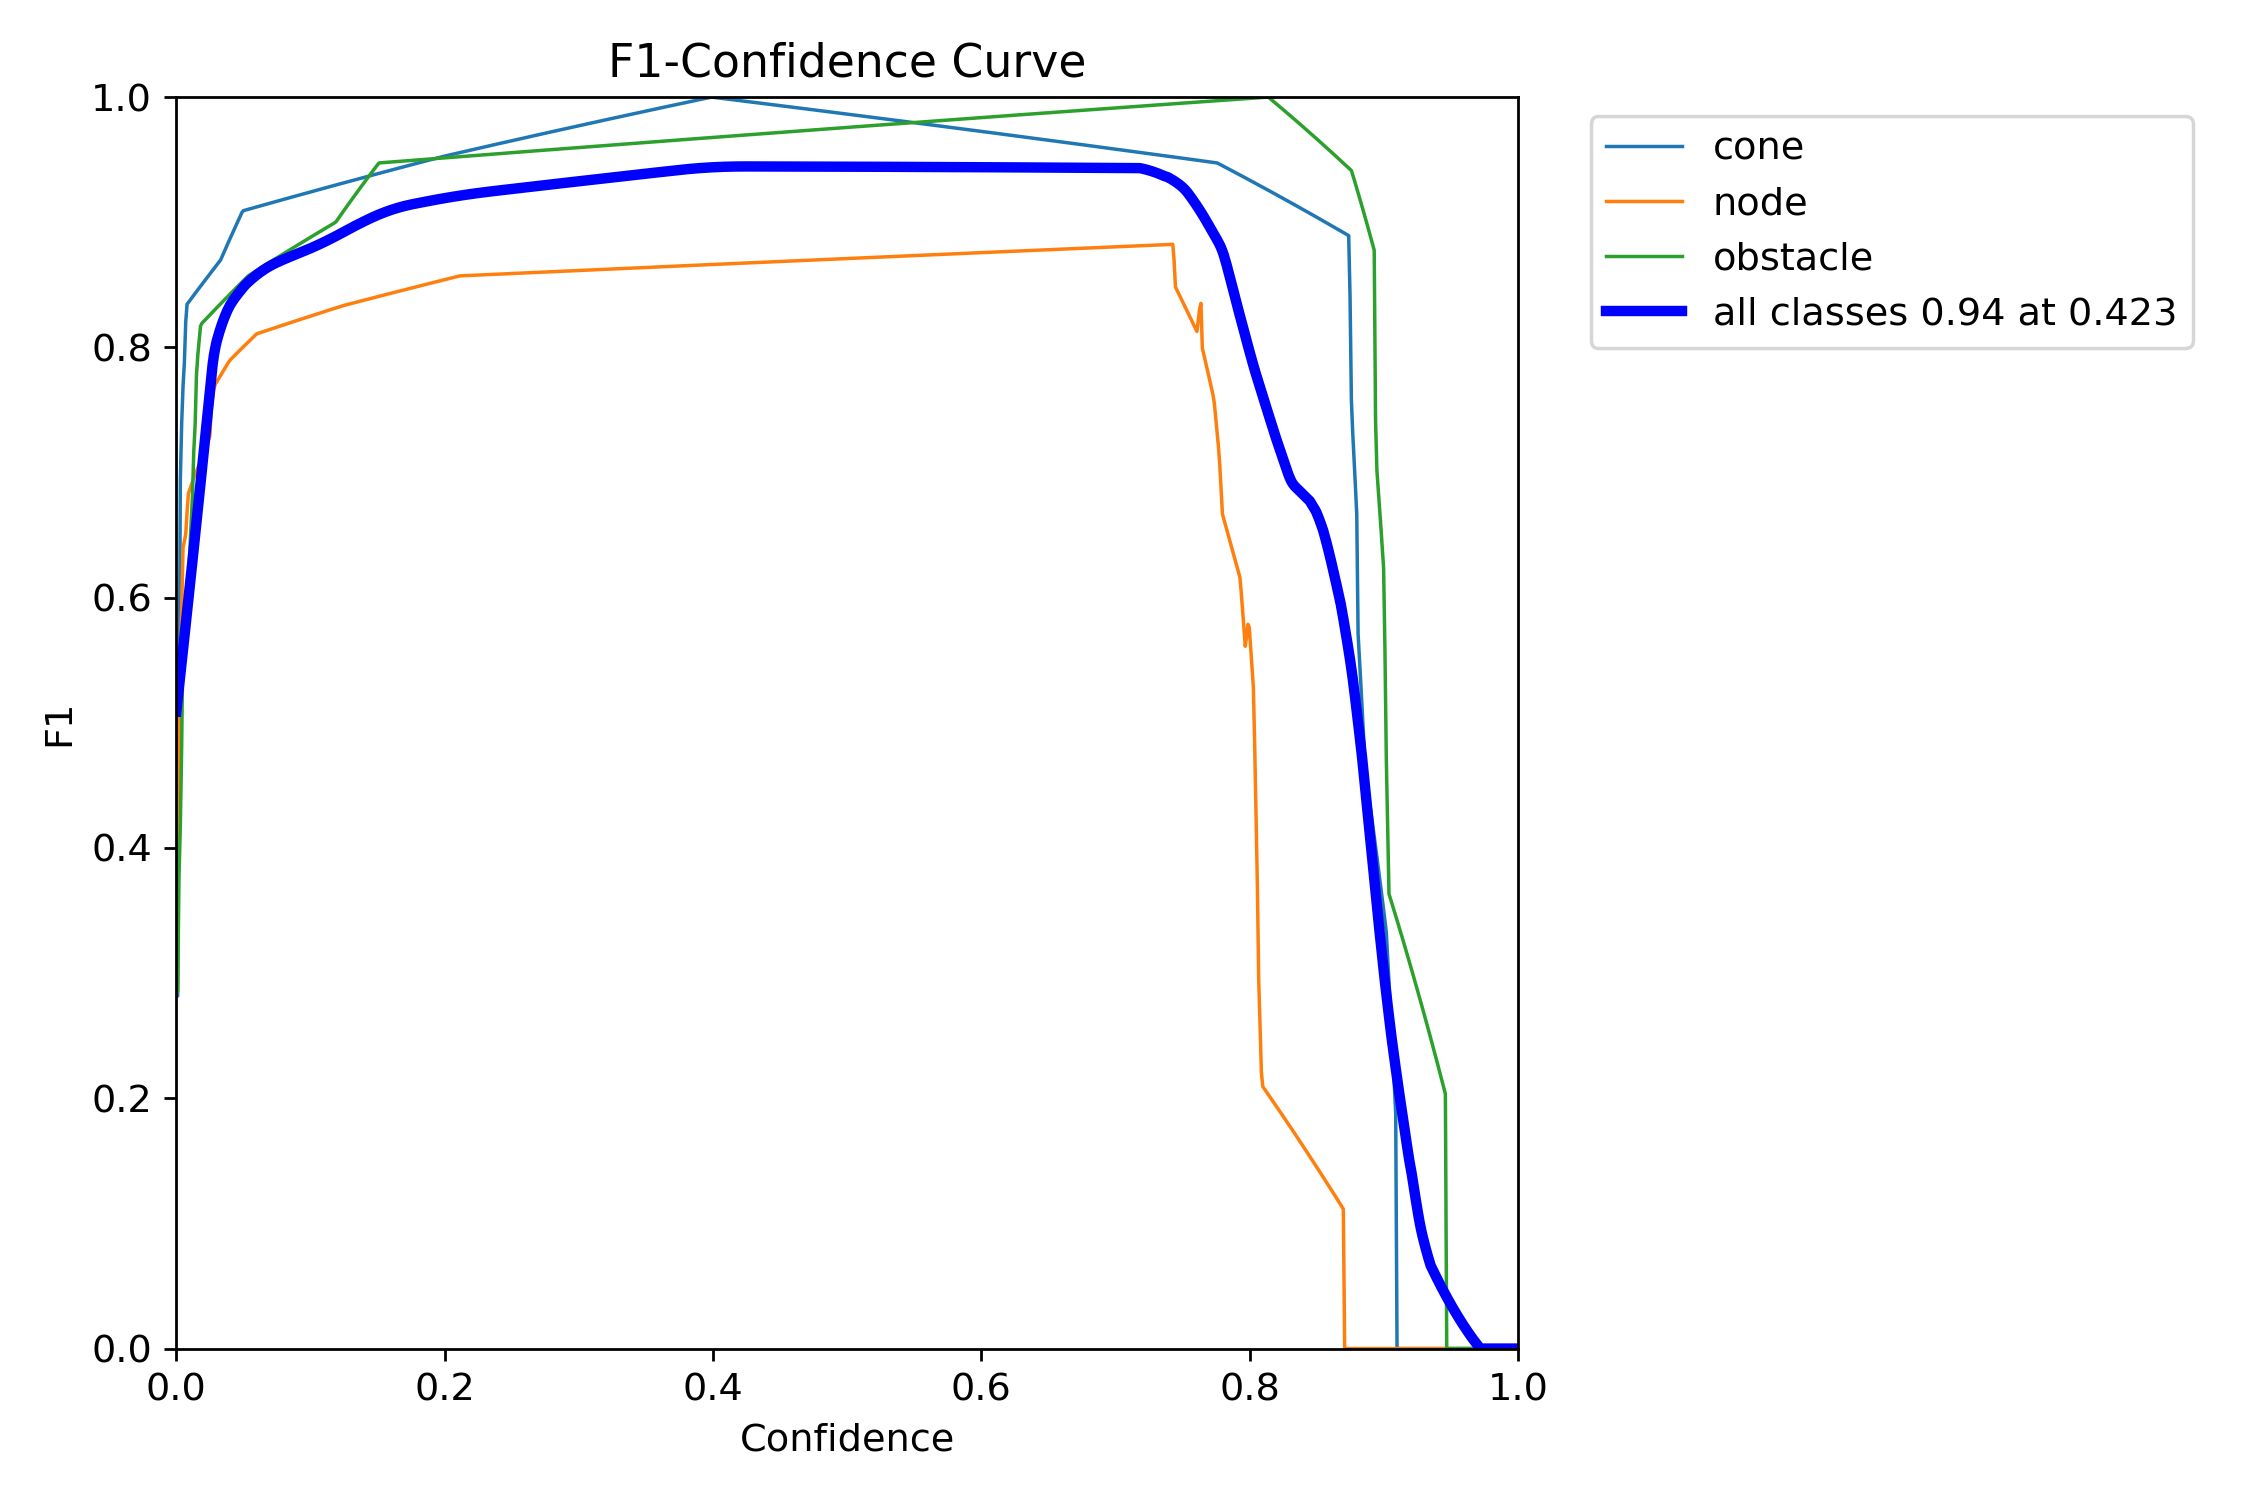
\includegraphics[width=\textwidth]{assets/IT/yolo/F1_curve.png}
    \caption{F1 Kurve}
    \label{fig:f1}
  \end{minipage}
  \hfill
  \begin{minipage}[b]{0.3\textwidth}
    \centering
    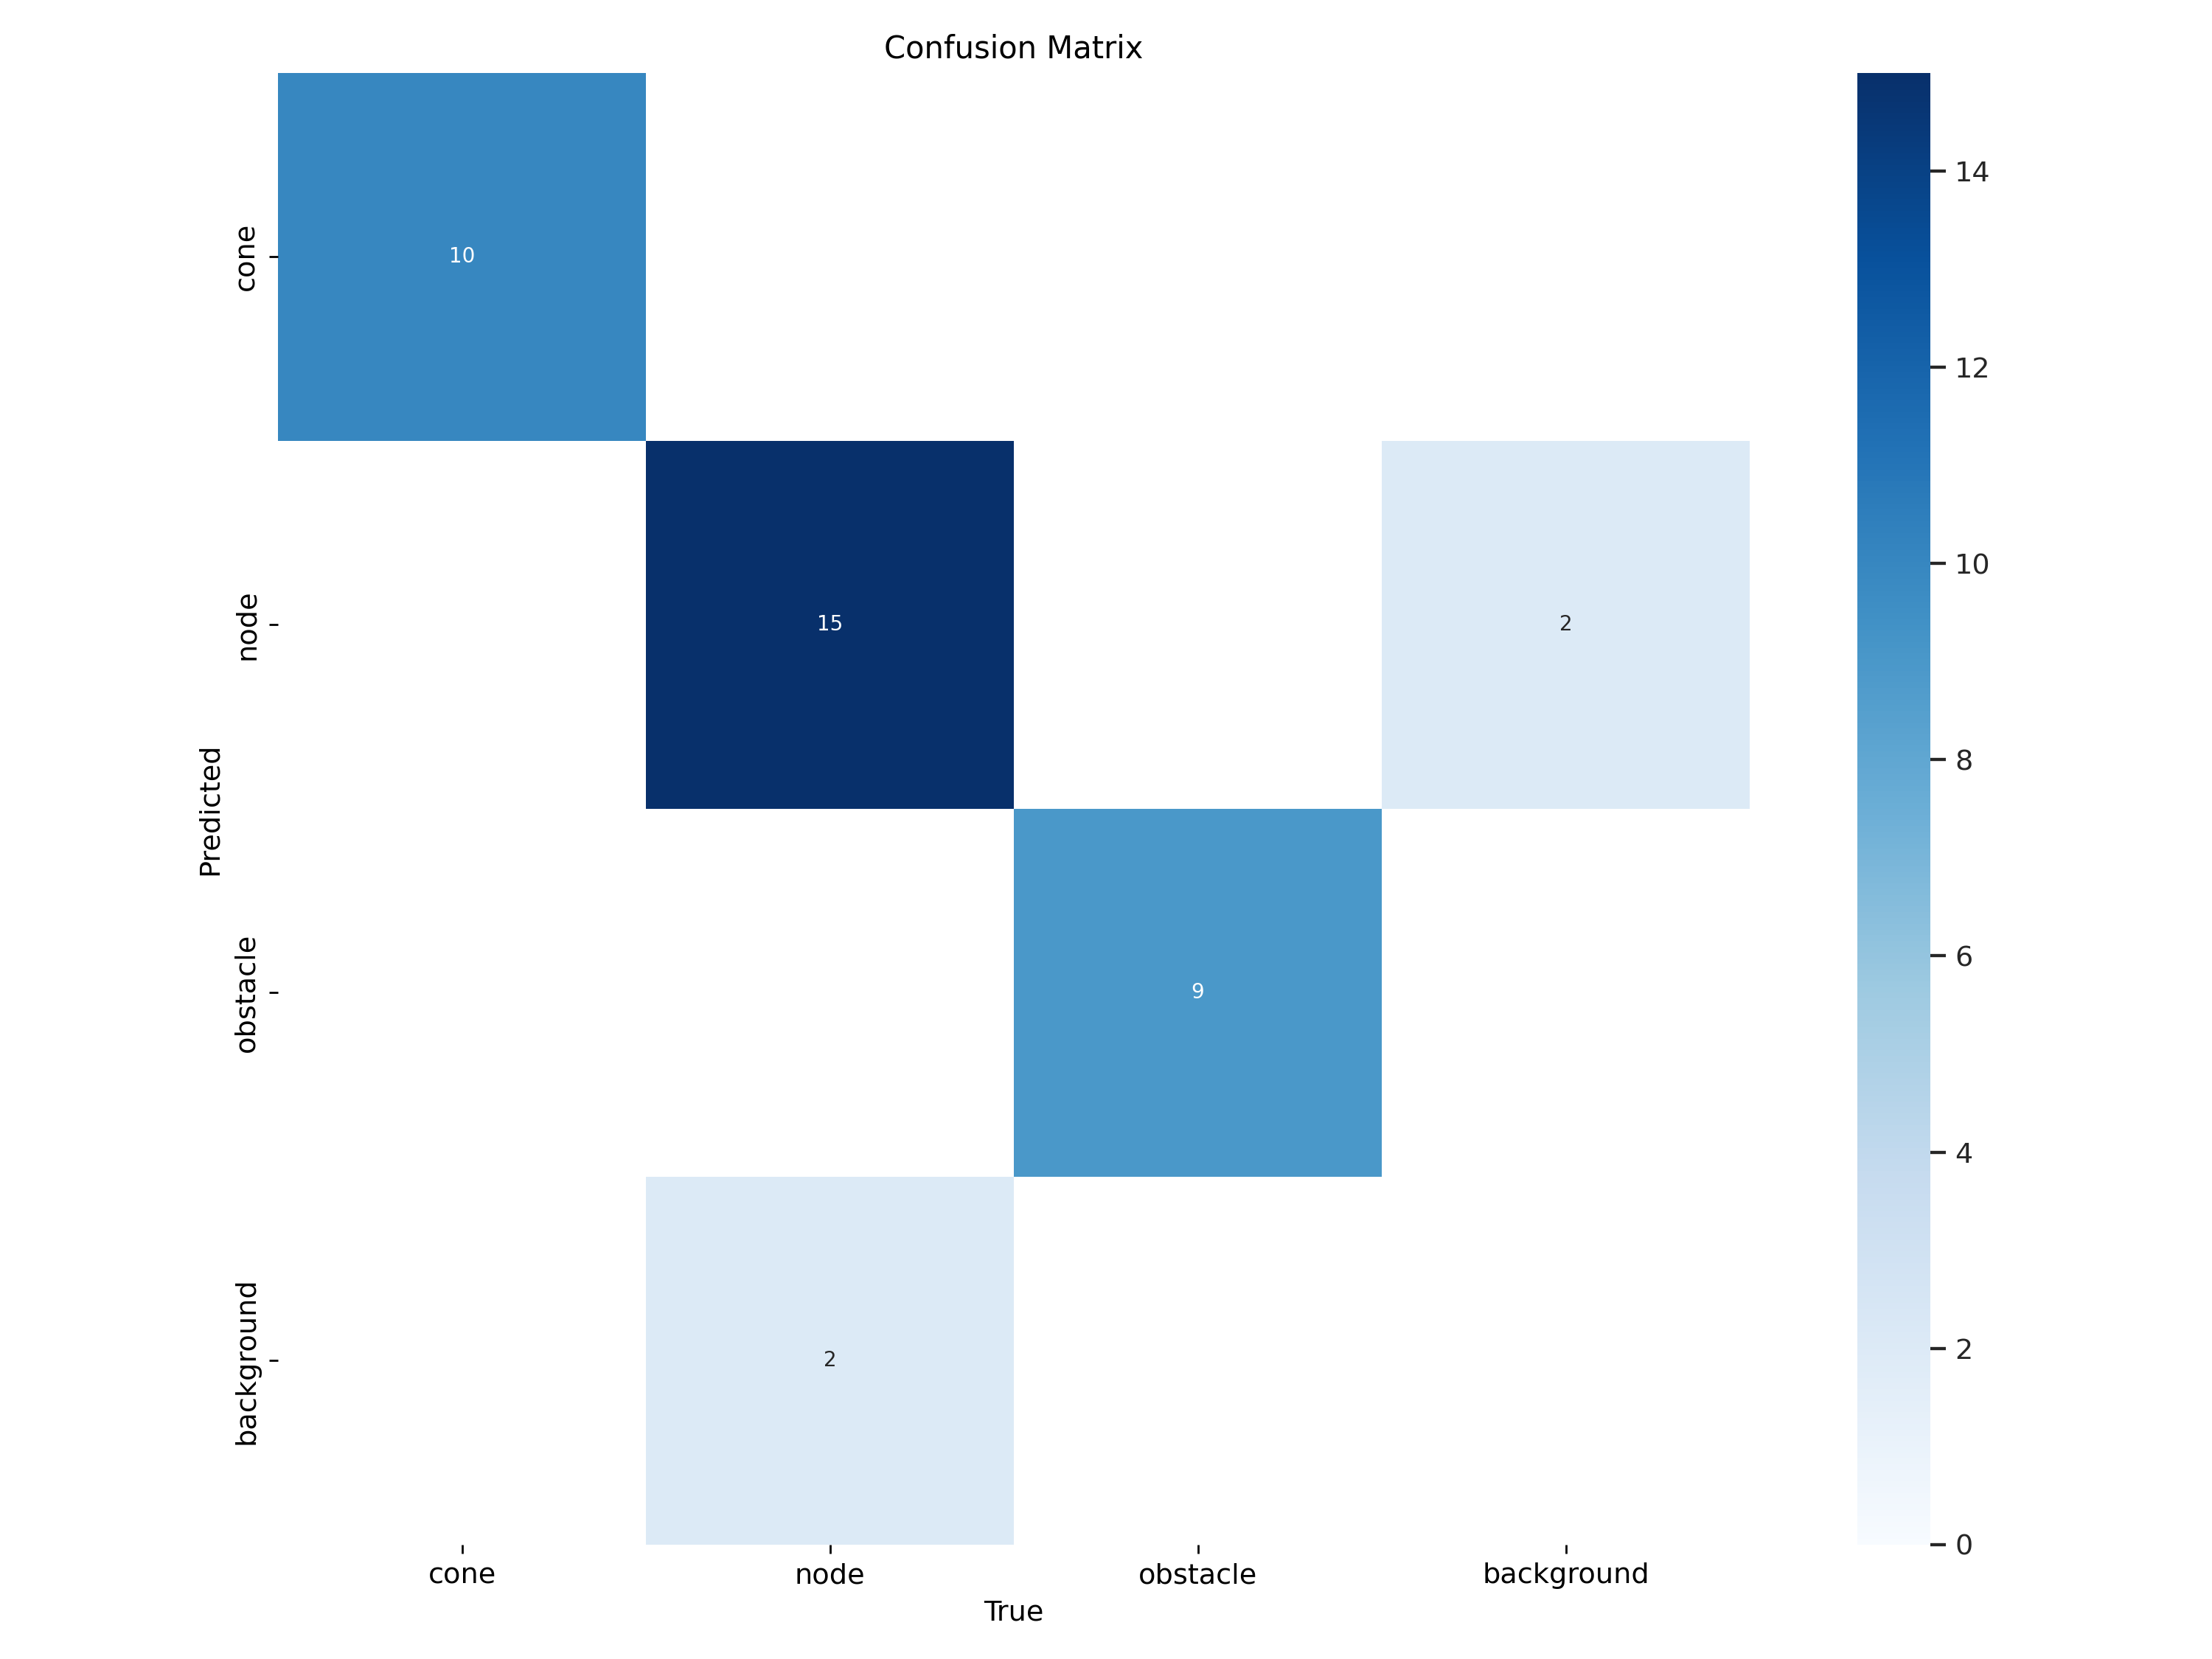
\includegraphics[width=\textwidth]{assets/IT/yolo/confusion_matrix.png}
    \caption{Confusion Matrix}
    \label{fig:conf-matrix}
  \end{minipage}
    \hfill
  \begin{minipage}[b]{0.3\textwidth}
    \centering
    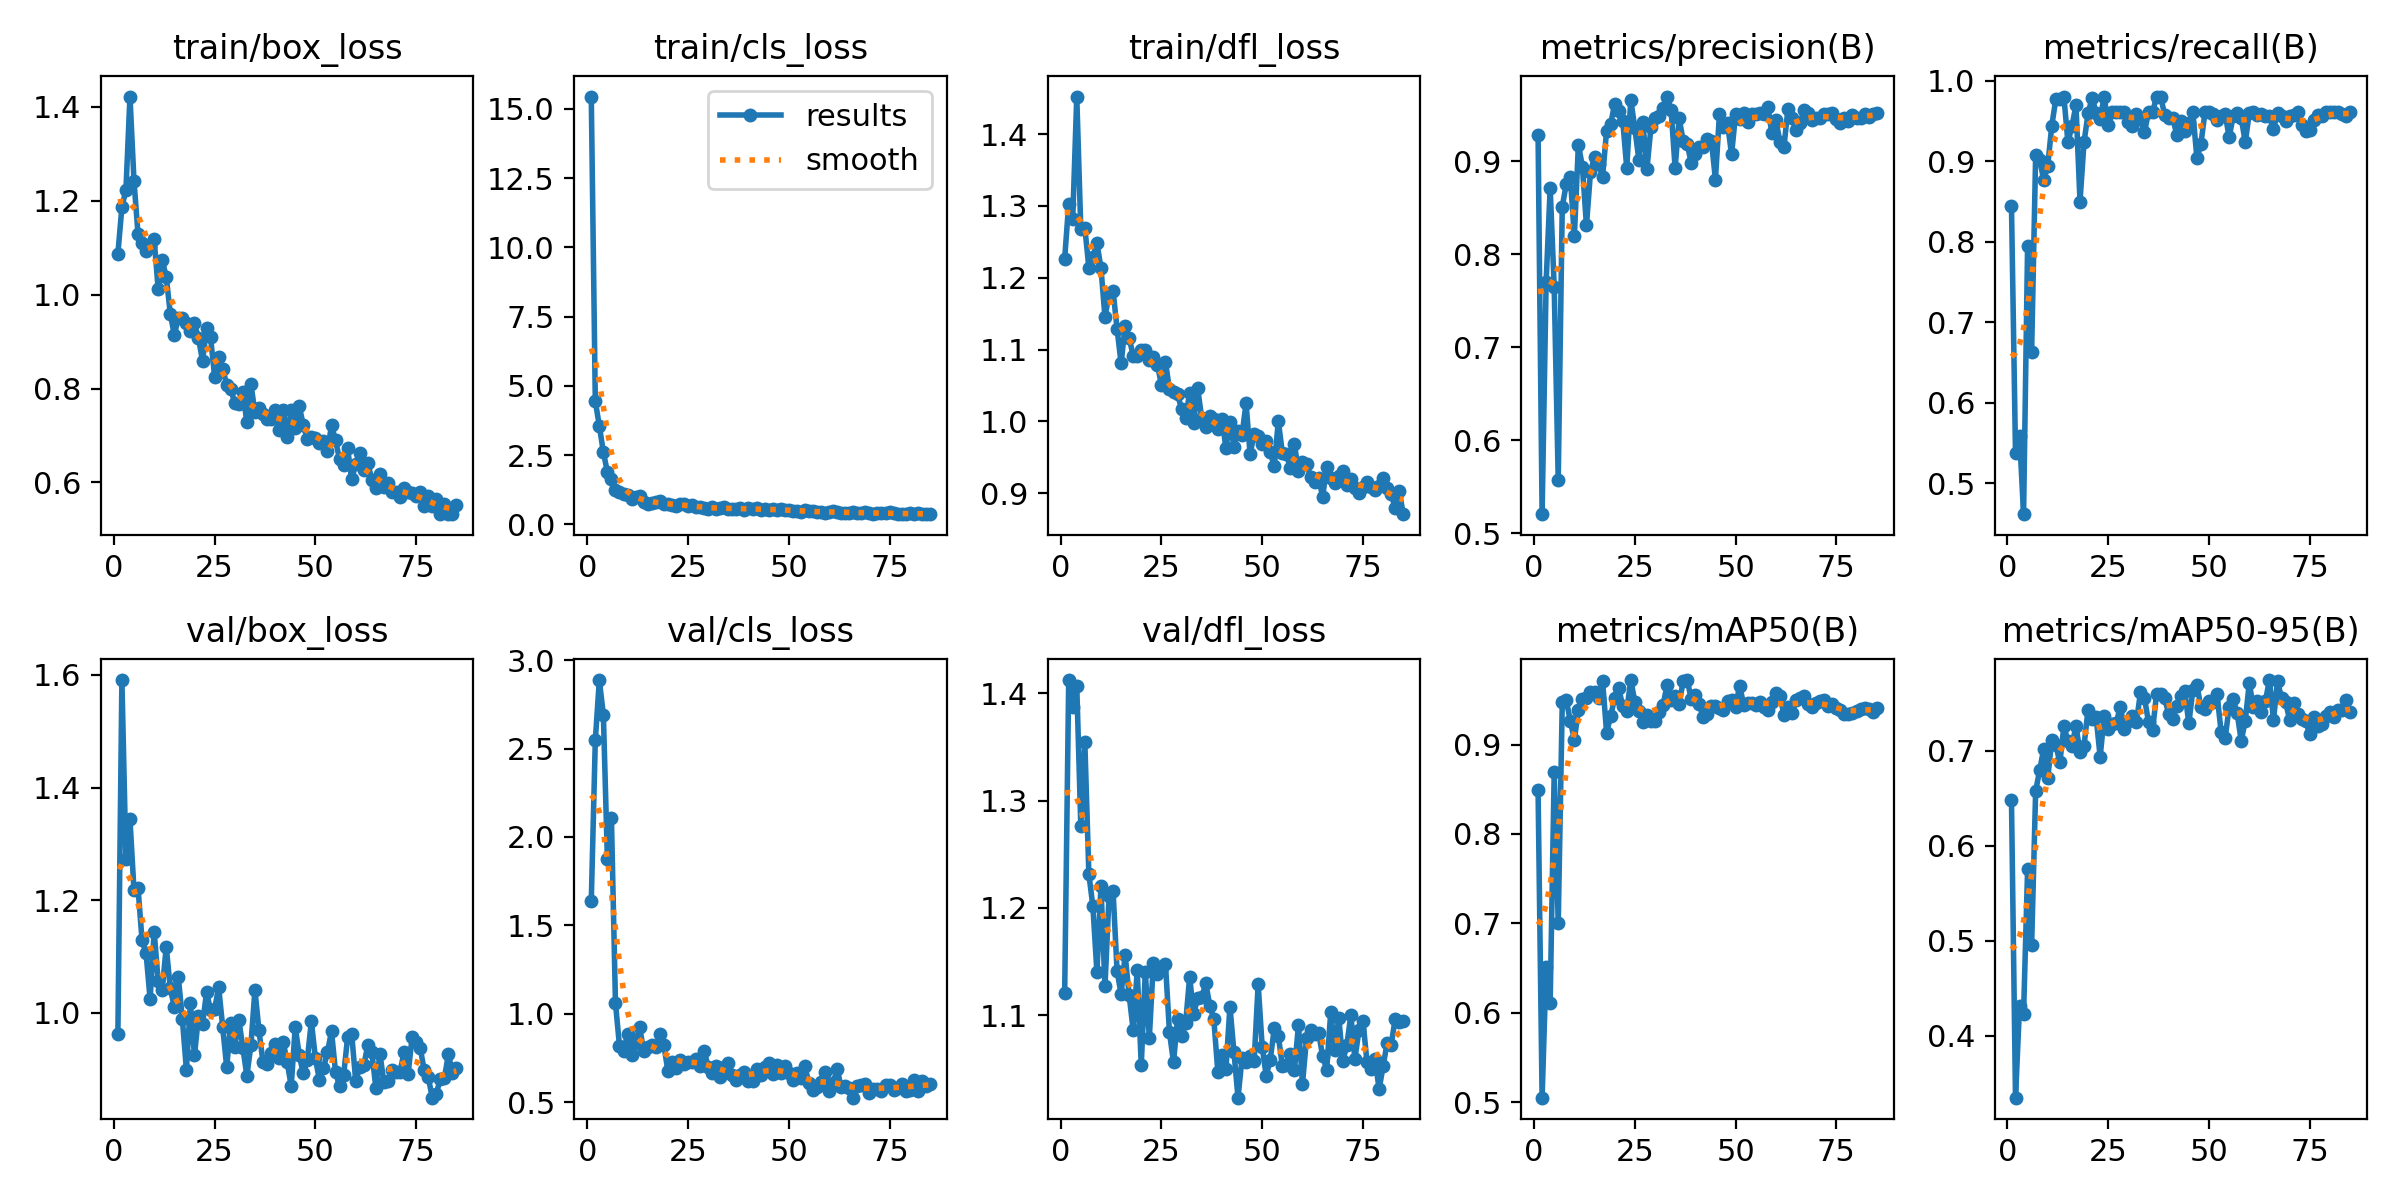
\includegraphics[width=\textwidth]{assets/IT/yolo/results.png}
    \caption{Lernverlauf}
    \label{fig:results-lernverlauf}
  \end{minipage}
\end{figure}

\subsubsection{YOLOv11 Model konvertieren}
\label{convert-yolo}

Es gibt Methoden, um die .pt Datei, die beim Trainieren von YOLO erstellt wird, zu transformieren in ein anderes Format, damit auf Embedded Systems und somit auch auf Raspberry Pi's schneller die Bilderkennung durchgeführt werden kann.

Drei Möglichkeiten wurden betrachtet und verglichen:
TODO add sources for each \& akronyum
\begin{enumerate}
    \item Caffe2: In der Vergangenheit sehr geeignet, heutzutages mit PyTorch zusammengefügt und existiert nicht mehr auf diese Weise.
    \item NCNN: Sehr gute Performance für ARM Geräte (u.a. Raspberry Pi), sehr wenig Abhängigkeiten, einfache Transformation.
    \item ONXX: Geeignet für  Cross-Plattform Fälle, gute Austauschbarkeit des Models, flexibel, viele Abhängigkeiten.
\end{enumerate}

Es wird NCNN gewählt, da dies perfekt für den Use Case mit einem Raspberry Pi passt. Das erstellte .pt File kann mit der ultralytics Bibliothek transformiert werden:

\begin{verbatim}
yolo export model=best.pt format=ncnn
\end{verbatim}

Das Resultat ist ein Ordner, der gleich verwendet werden kann, wie das .pt File. Mit der Transformation wurde das Risiko 3: 4 Minuten reichen nicht für einen Durchgang, weiter gemindert. Auf dem Raspberry Pi, kann die Bilderkennung pro Bild konstant unter einer Sekunde gehalten werden.

\subsubsection{Modelresultate auswerten}
\label{model-results}

Um die Modelresultate auszuwerten wurde das Model in den Ordner der Navigation kopiert und es wurde eine ObjectDetector Klasse und ein Object Enum erstellt, gezigt im Klassendiagramm \ref{fig:nav-object-detector}.

 \begin{figure}[H]
\centering
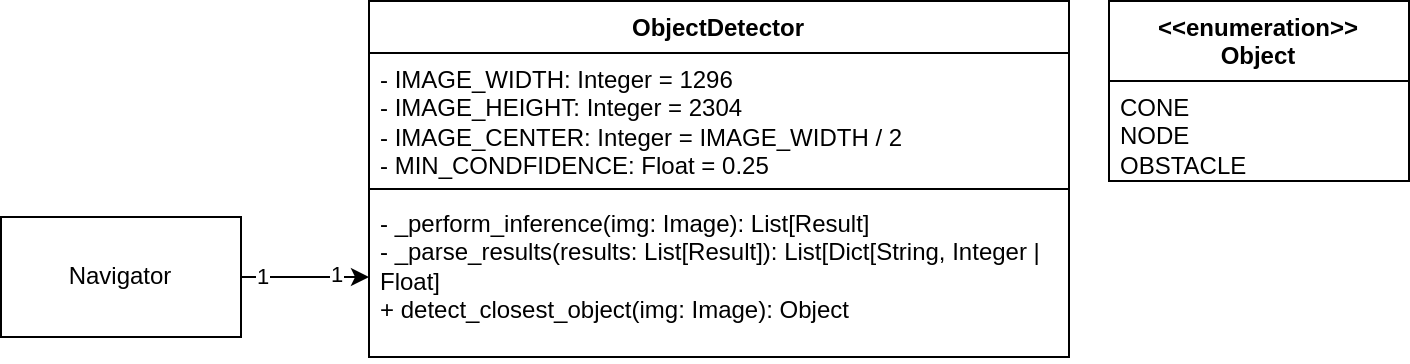
\includegraphics[width= \textwidth ]{assets/IT/robot-sw-architecture-object-detector.png}
\caption{Object Detector Modul}
\label{fig:nav-object-detector}
\end{figure}

Diese ObjectDetector Klasse ladet das Model bei der Instanzierung und wird aufgerufen, wenn ein Nachbarsknoten geprüft werden soll und führt einen Prozess von drei Schritten durch:

\begin{enumerate}
    \item Inference (Objekterkennung).
    \item Resultat parsen.
    \item Nächstes Objekte vor dem Roboter finden.
\end{enumerate}

Im Teil der Inference wird ein Bild an das Model gegeben. Dabei sollen nur die erkannten Objekte zurückgegeben werden, die mit einer definierten prozentualen Gewissheit erkannt wurden. Diese Gewissheit ist als Konstante definiert auf TODO WERT \& WIESO. \& falls Risiko damit vermindert (Falls erhoeht), Risiko 7

Diese Resultate werden dann geparsed, sodass alle erkannten Objekte mir ihrer ID, mit der Confidence, mit der sie erkannt wurden, und mit ihrem Standort auf dem Bild zurückgegeben werden.

Aus dieser Liste werden nun alle Objekte betrachtet, die sich auf der Mittellinie des Bildes befinden. Somit kann sichergestellt werden, dass nicht versehentlich Objekte, die sich nicht auf der Fahrbahn befinden, gespeichert werden und auch Risiko 7 (Objekte werden fälschlicherweise erkannt) kann so mitigiert werden. Die Mittellinie wird berechnet aus der Breite des Bildes. Die Objekte auf der Mittellinie werden sortiert nach ihren Koordinaten auf dem Bild. Das erste Element in dieser Liste ist das nächste Objekt zum Roboter. Die ID des Objektes, die vom Model zurückgegben wird, korrespondiert mit der ID des erstellten Enums, damit das erkannte Objekt als Enum zurückgegeben wird.

In folgenden Fällen wird nicht einfach das nächste Objekt zurückgegeben:

\begin{itemize}
    \item Falls das nächste Objekt eine Barriere und das zweitnächste eine Pylone ist. In diesem Fall wird zurückgegeben, dass eine Pylone das nächste Objekt ist, da dieser Knoten sowieso nicht befahrbar ist und aus dem internen Graph entfernt werden soll.
    \item Falls kein Objekt erkannt wurde, wird ein Knoten zurückgegeben. Es ist weniger wahrscheinlich, dass eine Barriere oder ein Pylon verpasst werden, als dass ein Knoten nicht erkannt wird. Somit wird Risiko 2 (Knoten werden nicht erkannt) behandelt. Der Ultraschall kann trotzdem Objekte noch erkennen, falls ein Objekt verpasst wurde. Es ist ein kleineres Problem ein Objekt zu verpassen, als sich eines einzubilden und fälschlicherweise Strecken zu entfernen. Durch den Ultraschall werden Risiko 12 und 1 (Objekte werden nicht erkannt) mitigiert.
\end{itemize}


Wie auf die einzelnen Objekte reagiert wird, ist in folgender Aufzählung beschrieben und ist gleich, wie in \acrshort{pren1} geplant.

\textbf{Pylonen erkennen}

Wird eine Pylone erkannt, wird der Knoten, der gerade geprüft wurde, inklusive alle Strecken dahin, aus dem internen Graphen entfernt.

\textbf{Knoten erkennen}

Wenn ein Knoten erkannt wird, dann geschieht nichts. Es wird interpretiert, dass sich kein Objekt auf diesem Weg befindet und die Strecke normal befahrbar ist.

\textbf{Barrieren erkennen}

Wird auf dem Bild eine Barriere erkannt, wird dies im internen Graphen gespeichert, indem die jeweilige Linie höher gewichtet wird, da es länger dauern wird diese zu überqueren.

\textbf{Entfernte Linien erkennen}

Die entfernten Linien werden erkannt, wenn die Winkel der ausgehenden Linien berechnet wird, Details dazu, gibt es in Kapitel \ref{outgoing-lines}. Die fehlende Linie wird aus dem internen Graphen entfernt.

\newpage
%%%%%%%%%%%%%%%%%Epic 11%%%%%%%%%%%%%%%%%%%%%%%%%%%%%%%%%%%%%%%%%%%%%%%%%%%%%%%
\subsection{Zieleingabe: Peripherie Ein- und Ausgabe}

In diesem Kapitel wird die Ein- und Ausgabe des Roboters thematisiert.
Dafür wurde auf dem Raspberry Pi ein Prototypen-HAT montiert, welcher die benötigten GPIO-Pins entsprechend der Abbildung \ref{fig:raspiheader-schema} auf Taster, Display und Buzzer verbindet.

\begin{figure}[H]
    \centering
    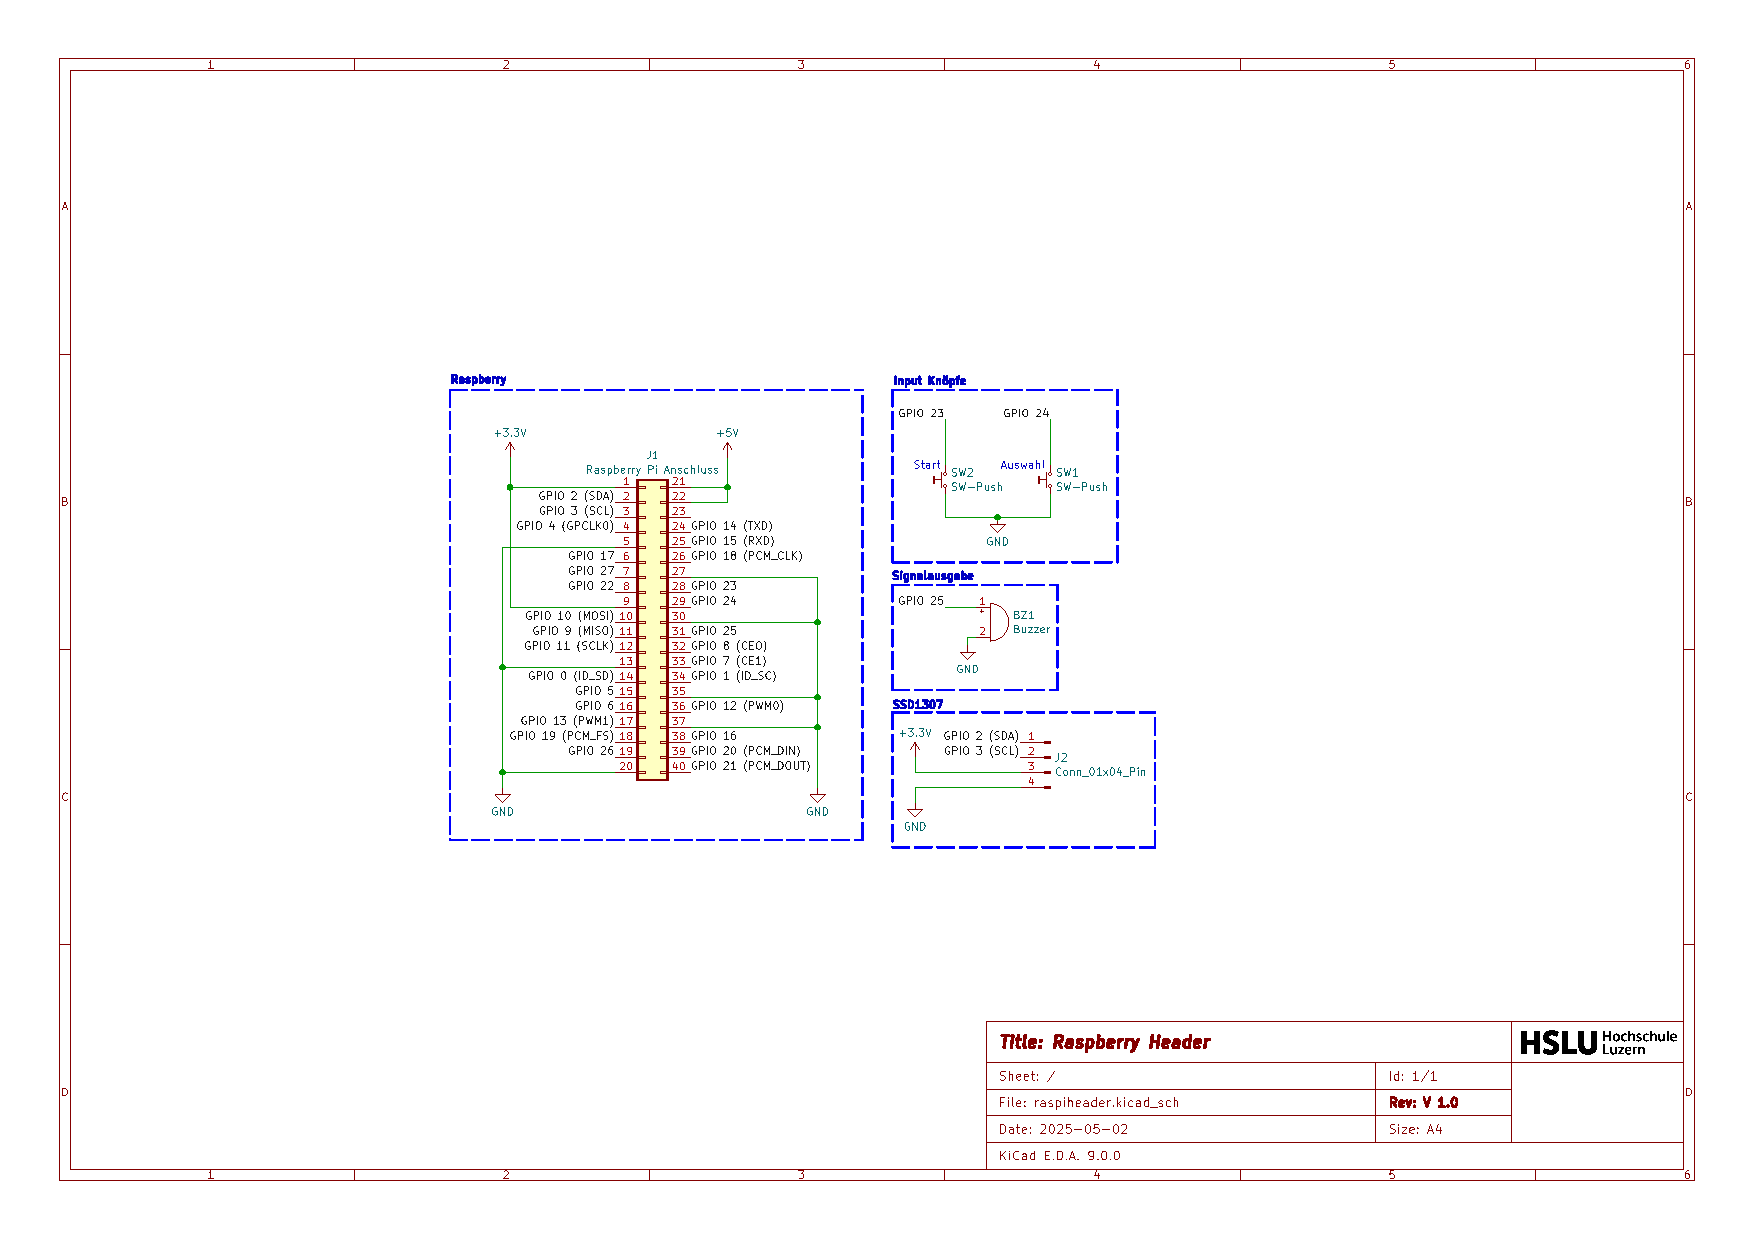
\includegraphics[width=\linewidth, trim=7.5cm 6cm 10cm 6cm, clip]{assets/ET/PCB/raspiheader.pdf}
    \caption{Raspberry Pi HAT Schema}
    \label{fig:raspiheader-schema}
\end{figure}

TODO LUKAS: insert image of raspberry pi hat assembled
\begin{figure}[H]
    \centering
    
\includegraphics[width=0.5\linewidth]{assets/placeholder.png}
    \caption{Raspberry Pi HAT}
    \label{fig:raspiheader-assembly}
\end{figure}

\subsubsection{Peripherie Eingabe}
\label{zieleingabe}

\textbf{Zielknopf}

Die Zieleingabe wird dazu verwendet, um vor dem Start den geforderten Zielknoten auszuwählen. Bei Knopfdruck wird der gewählte Zielknoten durchgeschaltet, dies in der Reihenfolge A --> B --> C und dann wieder von vorne. So wird nur ein Taster benötigt, um zwischen den drei Zielen zu wechseln. Das Gewählte Ziel ist stets im Display (\ref{peripherie-display}) ersichtlich.

\textbf{Startknopf}

Der zweite Taster ist der Startknopf. Dieser wird nach der Eingabe des Zielknoten gedrückt, nach einer kurzen Wartezeit wird dann der Start initialisiert und der Roboter fängt an den Graphen Richtung Zielknoten zu traversieren.

Durch die einfache Zweitaster-Bedienung, und das ablesbare Display ist das Aufstellen sowie wählen des Zielknoten sehr gut unter 1 Minute möglich. 

\subsubsection{Peripherie Ausgabe}

\textbf{Display}\label{peripherie-display}

Das Display zeigt stets den aktuellen gewählten Zielknoten an, so kann einfach überprüft werden, welcher Zielknoten gewählt wird, bevor der Roboter gestartet wird. 
Zusätzlich wird der Status sowie die Laufzeit des Roboters dargestellt. Dadurch muss nicht separat eine Stoppuhr verwendet werden. Die Laufzeit wird automatisch beim erreichen des Zielknoten gestoppt und bleibt ablesbar.

TODO LUKAS: insert image of Display
\begin{figure}[H]
    \centering
    
\includegraphics[width=0.5\linewidth]{assets/placeholder.png}
    \caption{Raspberry Pi HAT}
    \label{fig:raspiheader-display}
\end{figure}


\textbf{Buzzer}\label{peripherie-buzzer}

Der Buzzer ertönt sobald der Zielknoten erreicht wurde. Somit wird dem Bediener und Publikum vermittelt, dass der Roboter seine Traversierung beendet hat, und sich am Zielknoten befindet.
